\documentclass{ltjarticle}
\usepackage{graphicx} % Required for inserting images
\usepackage{setspace} \doublespacing
\usepackage[margin=35truemm]{geometry}
\usepackage{hyperref}
\hypersetup{
    colorlinks=true,
    linkcolor=blue,
    filecolor=blue, 
    urlcolor=blue,
    pdftitle={Overleaf Example},
    pdfpagemode=FullScreen,
    }
\usepackage{booktabs}
\usepackage{caption}
\usepackage{amsmath}
\usepackage{rotating}
\renewcommand{\figurename}{Figure}
\renewcommand{\tablename}{Table}



\title{Topics in Econometrics F\\Final Project: Replication of Mian et al. (2017)\footnote{Atif Mian, Amir Sufi, Emil Verner, Household Debt and Business Cycles Worldwide, \textit{The Quarterly Journal of Economics}, Volume 132, Issue 4, November 2017, Pages 1755-1817, \href{run: https://doi.org/10.1093/qje/qjx017}{https://doi.org/10.1093/qje/qjx017}}}
\author{Kosuke Sato}
\date{October 2023}

\begin{document}

\maketitle

\section*{Abstract}
This paper investigates the relationship between the household debt to GDP ratio and GDP growth. While GDP grows in high ratio during the household debt booms, economic forecasters tend to overpredict the GDP growth at the end of booms. They used an unbalanced panel for 30 countries from 1960 to 2012 to show the negative relation between the growth of household debt to GDP and subsequent output growth in several years. While the paper consists of ten sections, the main result is the third one, and the rest ones discuss the underlying theories and confirm them empirically. Therefore, I challenged to replicate the first to third sections, and discuss the results and theoretical background of them. The replication code is uploaded on my github repository: \href{run:https://github.com/1414satok/Mian-et-al-2017}{https://github.com/1414satok/Mian-et-al-2017}.
\newpage

\section{Introduction}
After the Great Recession, many researchers are interested in the relationship between household debt and the macroeconomy. The Great Recession was caused by the overpredict of GDP growth in a household debt boom, and it implied that the increase in household debt predicts the severity of the downturn. 

They investigated the relation between household debt and business cycle, and found that a shock to the household debt to GDP provoke a three to four year rise of household debt using VAR. Moreover, they showed that, during this boom, the consumption to GDP ratio, imports of consumption goods, and GDP rise, but GDP subsequently falls after a few years. 

After the empirical studies, they confirm the results theoretically. The background theories about the rise in household debt can grouped into two categories. The first is models based on credit demand shocks, and the second is those based on credit supply shocks. And the results can also be confirmed with the macroeconomic frictions worsening the economic downturn that follows the rise in debt.

The first theory, models based on credit demand shocks, contradicts the results, because such a model implies the positive correlation between contemporaneous changes in household debt and subsequent economic growth, because households borrow because they expect the improvement of economy. Moreover, the theory yields interest rate gets higher when borrowers become optimistic. And this is not consistent with the results either.
The second theory is more consistent with the result. They fond that a measure of credit supply shocks caused by the quality of credit originated to low credit quality firms is positively correlated with household debt booms. They show that household debt rise predict lower subsequent growth.

And they also mention about the source of the increase in credit supply. During booms, economic leaders tend to ignore downside risks and willing to make credit more available cheaply. They showed that economic forecasters served from international economic organization over-forecast GDP growth at the end of booms. 

Furthermore, at the end of credit booms, frictions in nominal measures and economic policy worsen the decline in subsequent growth. Similarly, credit booms make resources less available, and so unemployment rate get increase in household debt booms.

Household debt booms also affect badly the global dimension of economy. A rise in household debt to GDP causes a subsequent decrease in the trade deficit. As a result, net exports decline and it has negative effect on the household debt boom on consumption and investment. They show that countries whose economy is more correlated with a household debt to GDP cycle than global debt cycle undergo a stronger decline in subsequent output growth after a household debt boom.

The following part is structured same as the original paper. In Section 2, I introduce the dataset and summary the statistics. Section 3 shows the main results, and Section 4 discusses the theories underlying behind the results.

\section{Data and Summary Statistics}
\subsection{Data}
They employ a country level unbalanced panel data from 1960-2012. This data set includes the information on household and nonfinancial firm debt to GDP, national accounts, unemployment, professional GDP forecasts, credit spread, and international trade. The data are annual and include 30 countries from both of developed and emerging. The level of household and nonfinancial firm debt are measured as the household debt to GDP ratio and nonfinancial firm debt to GDP ratio, which are referred as $d_{it}^{HH}=\frac{D_{it}^{HH}}{Y_{it}}$ and $d_{it}^{F}=\frac{D_{it}^{F}}{Y_{it}}$. They measure the change in household and firm debt from year $t-k$ to year $t$ as $\Delta_{k} d_{it}^{HH} $ and $\Delta_{k}d_{it}^{F} $.

The data used in our replication is referred from the Harvard Dataverse\footnote{\hyperlink{https://dataverse.harvard.edu/dataset.xhtml?persistentId=doi:10.7910/DVN/FEDKGY}{https://dataverse.harvard.edu/dataset.xhtml?persistentId=doi:10.7910/DVN/FEDKGY}}. This page serves the replication data used in the original paper, and the matlab and stata code to make the tables and figures. With this data, I write the code in R to replicate the results.

\begin{table}[hbtp]
    \small
    \begin{center}
        \caption{Summary Statistics}
        \label{table1}
        \begin{tabular}{rrrrrr}
              \hline
              \hline
             & N & Mean & Median & Std. dev. & $\frac{\text{Std. dev.}}{\text{Std. dev.} (\Delta y)} \\ 
              \hline
            $\Delta y$ & 695 & 2.90 & 3.08 & 2.98 & 1.00 \\ 
            $\Delta_{3}y$ & 695 & 8.40 & 8.65 & 6.56 & 2.21 \\ 
            $\Delta d^{Private}$ & 695 & 3.11 & 2.52 & 6.96 & 2.34 \\ 
            $\Delta_{3}$ d^{Private} & 695 & 8.52 & 7.28 & 16.04 & 5.39 \\ 
            $\Delta d^{HH}$ & 695 & 1.62 & 1.33 & 2.56 & 0.86 \\ 
            $\Delta_{3}d^{HH}$ & 695 & 4.58 & 3.68 & 6.24 & 2.10 \\ 
            $\Delta d^{F}$ & 695 & 1.48 & 1.04 & 5.66 & 1.90 \\ 
            $\Delta_{3}d^{F}$ & 695 & 3.89 & 3.11 & 12.21 & 4.10 \\ 
            $\Delta_{3}d^{Gov}$ & 627 & 1.73 & 1.16 & 9.92 & 3.33 \\ 
            $\Delta_{3}d^{Netforeign}$ & 636 & -0.57 & 1.30 & 15.01 & 5.04 \\ 
            $\Delta_{3}c$ & 678 & 2.81 & 2.90 & 2.84 & 0.95 \\ 
            $\Delta_{3}c^{dur}$ & 469 & 4.91 & 5.35 & 9.27 & 3.12 \\ 
            $\Delta_{3}c^{nondur}$ & 469 & 1.53 & 1.47 & 2.53 & 0.85 \\ 
            $\Delta\frac{C}{Y}$ & 690 & -0.06 & -0.01 & 1.17 & 0.39 \\ 
            $\Delta{i}$ & 678 & 2.66 & 3.67 & 10.79 & 3.63 \\ 
            $\Delta{g}$ & 688 & 2.84 & 2.60 & 2.79 & 0.94 \\ 
            $\Delta{x}$ & 695 & 8.64 & 9.30 & 12.29 & 4.13 \\ 
            $\Delta{m}$ & 695 & 8.08 & 9.55 & 13.87 & 4.66 \\ 
            $\Delta\frac{NX}{Y}$ & 695 & 0.14 & -0.01 & 2.11 & 0.71 \\ 
            $\Delta\frac{CA}{Y}$ & 648 & 0.08 & -0.02 & 2.29 & 0.77 \\ 
            $\Delta s^{XC}$ & 695 & -0.15 & -0.07 & 1.80 & 0.61 \\ 
            $\Delta s^{MC}$ & 695 & 0.16 & 0.15 & 1.67 & 0.56 \\ 
            $\Delta reer$ & 614 & -0.03 & 0.59 & 6.75 & 2.27 \\ 
            $\Delta u$ & 669 & 0.08 & -0.01 & 1.08 & 0.36 \\ 
            $\Delta_{3}u$ & 662 & 0.19 & -0.01 & 2.43 & 0.82 \\ 
            $\Delta{3}y_{t+3|t}^{WEO}$ & 484 & 9.41 & 8.60 & 3.76 & 1.26 \\ 
            $\Delta_{3}(y_{t+3}-y_{t+3|t}^{WEO}$ & 484 & -2.53 & -1.79 & 5.35 & 1.80 \\ 
            $\Delta_{3}\ln(P^{Housing})$ & 514 & 6.56 & 7.16 & 17.42 & 5.85 \\ 
            $spr^{real}$ & 622 & 0.43 & 0.40 & 2.11 & 0.71 \\ 
            $spr^{MS}$ & 517 & 1.15 & 0.99 & 1.52 & 0.51 \\ 
            $spr^{corp}$ & 460 & 0.76 & 0.65 & 1.03 & 0.35 \\ 
               \hline
               \hline
        \end{tabular}
    \end{center}
    \begin{tablenotes}
        \small
        \item \textit{Notes}: Log changes and ratio are multiplied by 100. $\Delta$ and $\Delta_{3}$ denote one-year and three-year changes, respectively. $y$, $d^{Private}$, $d^{Private}$, $d^{HH}$, $d^{F}$, $d^{Gov}$, $d^{Netforeign}$, $c$, $c^{dur}$, $c^{nondur}$, $\frac{C}{Y}$, $i$, $g$, $x$, $m$, $\frac{NX}{Y}$, $\frac{CA}{Y}$, $s^{XC}$, $s^{MC}$, $reer$, $u$,  $y_{t+3|t}^{WEO}$, $\ln(P^{Housing})$, $spr^{real}$, $spr^{MS}$, and $spr^{corp}$ denote log real GDP, private nonfinancial debt to GDP, household debt to GDP, nonfinancial firm debt to GDP, government debt to GDP, the change in net foreign liabilities (sum of current account deficits to GDP), log real consumption ,  log real durable consumption, log real nondurable consumption, consumption to GDP, log real investment, log real government consumption, log nominal exports, log nominal imports, net exports to GDP, current account to GDP, the share of consumption exports to total exports, the share of consumption imports to total imports, log real effective exchange rate, the unemployment rate, the IMF Fall \textit{World Economic Outlook} time $t$ forecast of growth from $t$ to $t+3$, the log real house price index, the real 10-year government bond yield spread with respect to the United States, mortgage-sovereign spread, and the corporate-sovereign spread, respectively. This note refers the foot note in the table I of the original paper.
    \end{tablenotes}
\end{table}

\subsection{Summary Statistics}
Table \ref{table1} shows the summary statistics for the change in total private, household, and nonfinancial firm debt to GDP and the other variables\footnote{I use the same name of variable to avoid using misleading names}. Their empirical study uses both of first- and third-order difference.

\section{Household Debt, Firm Debt, and Economic Growth}
Their study investigates the relationship between household debt, firm debt, and economic growth. First, the research focuses on the full dynamic relation between debt and growth, followed by single-equation specification.
\subsection{Full Dynamic Relation}
Their first research employ a recursive VAR specification with impulse responses from a Cholesky identification scheme to clarify the full dynamic relation between debt and GDP growth. Their VAR model includes three variables; the level of household debt to GDP, nonfinancial firm debt to GDP, and log real GDP, which are referred as $\mathbf{Y}_{it}=(y_{it},d_{it}^{F},d_{it}^{HH}) $. Those variables are normalized by one-year-lagged GDP to avoid capturing innovations to GDP in the debt equations. Without normalized, the growth of debt has a risk to capture economically meaningless growth if the debt improve from a small base.

The VAR in levels with country fixed effects can be written as

\begin{equation*}
    \mathbf{AY}_{it}=\mathbf{a}_{i}+\sum_{j=1}^{p}\alpha_{j}\mathbf{Y}_{it-j}+\epsilon_{it}\nonumber
\end{equation*}

where $\mathbf{a}_{i}$ is a vector of country fixed effects and $\epsilon_{it}$ is an $n\times1$ vector of structural shock with $E[\epsilon_{t}\epsilon_{t}^{top}]=I, E[\epsilon_{t}\epsilon_{s}]=0 $ for $s\ne t$. They specify $p=5$ based on the Akaike information criterion.
The reduced form representation is given by
\begin{equation}
    \label{eq1}
    \mathbf{Y}_{it}=\mathbf{c}_{i}+\sum_{j=1}^{p}\delta_{j}\mathbf{Y}_{it-j}+\mathbf{u}_{it}
\end{equation}
where $\mathbf{S}=\mathbf{A}^{-1}$, $\mathbf{c}_{i}=\mathbf{S}\mathbf{a}_{i} $, $\delta_{j}=\mathbf{S}\alpha_{j} $, and $\mathbf{u}_{it}=\mathbf{S}\epsilon_{it} $ is the vector of reduced-form shocks with $E[\mathbf{u}_{it}\mathbf{u}_{it}^{\top}]=\mathbf{S}\mathbf{S}^{\top}=\Sigma $. When applying Cholesky decomposition, they set the structural shocks as real log GDP, nonfinancial debt to lagged GDP, and household debt to lagged GDP, in this order.

They estimate the reduced form VAR on the ful sample. When calculating the standard error, they employ an iterative bootstrap procedure to correct for potential Nickell bias from the inclusion of country fixed effects $\mathbf{a}_{i}$.

\begin{figure}[h]
    \begin{center}
        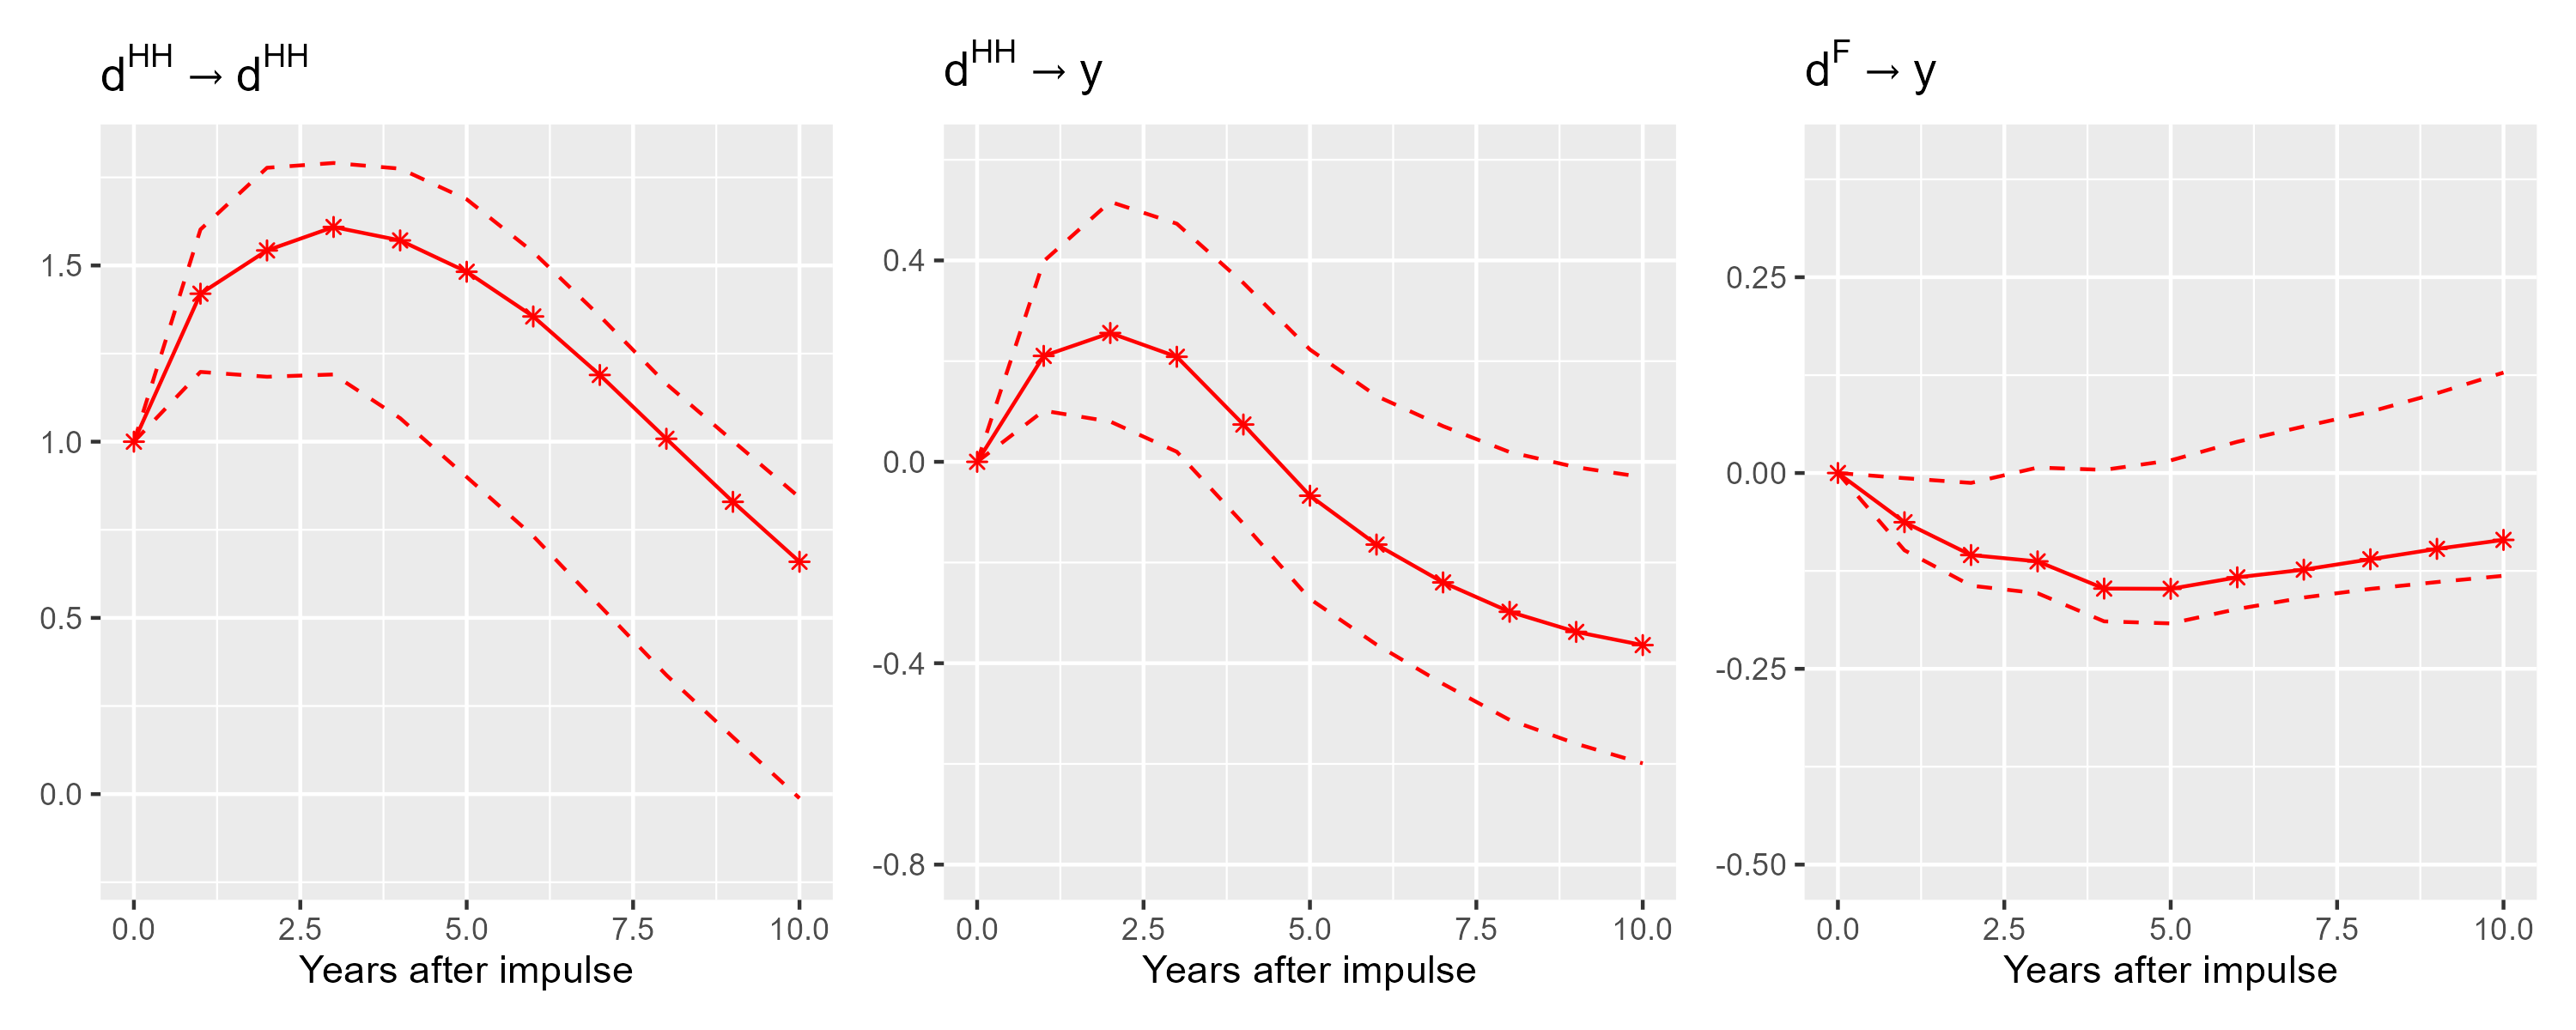
\includegraphics[scale = 0.5]{Figure1.png}
        \caption{}{Impulse Responses from a Recursive VAR in Real GDP, Nonfinancial Firm Debt, and Household Debt}
        \label{fig1}
    \end{center}
    \begin{tablenotes}
        \small
        \item \textit{Notes}: This figure shows impulse responses from a three variable VAR in log real GDP, firm debt to lagged GDP ratio, and household debt to lagged GDP ratio. The left panel shows the response of the household debt response to the shock of itself. The middle panel shows the real GDP growth response to the shock of household debt. The right panel shows the real GDP growth response to the shock of firm debt. The shocks are identified with a Choldesky decomposition with the ordering $\left(y_{it}, d_{it}^{F}, d_{it}^{HH}\right) $. The impulse response is estimated with the country level fixed effects. The reduced-form VAR coefficients are corrected for Nickell bias with an iterative bootstrap procedure. Dashed line shows 95\% confidence intervals computed by the wild bootstrap for the cross sections of residuals.
    \end{tablenotes}
\end{figure}

The result is shown in figure \ref{fig1}. There are three impulse responses. The center solid line shows the point estimates of impulse response, and the side dased lines shows the 95\% confidence interval of estimates.  The left panel shows the response of household debt to a shock to itself. This result can be interpreted as the length of a credit boom in the data. After a shock, household debt expands for three years, after when it reverts. In five years from the peak, household debt returns to the initial level. 

The middle panel shows the response of real GDP to a shock to household debt. In short-run, a shock of household debt has a positive effect on the GDP growth. However, it does not last as long as five years, and after that it returns to the initial level. From 6 to 10 years after the shock, the GDP become less than its starting point. However, they focus on the medium-run impact instead of long-run impact in this paper. The theory they employed in the following section can explain the effect of credit shocks on business cycle fluctuations. 

The right panel shows the impulse response of GDP to a shock to nonfinancial firm debt. The shock of firm debt immediately provoke the negative reaction of GDP. After 5 years the effect of a rise in firm dent reverts. In the following section, they found that firm and household debt shocks have statistically distinct effects on GDP growth in the short- and medium-run.

\begin{table}[h]
    \small
    \begin{center}
        \caption{}{Credit Expansion and Contermporaneous and Future Three-Year GDP Growth}
        \label{table2}
        \begin{tabular}[t]{lccccccc}
            \toprule
            & \multicolumn{7}{c}{Dependent variable: $\Delta_{3}y_{it+k}, k=-1,0,\cdots,5$} \\
            \cline{2-8}
              & (1) & (2) & (3) & (4) & (5) & (6) & (7)\\
            \midrule
            $\Delta_{3}d_{it-1}^{HH} $ & \num{0.176}* & \num{0.121} & \num{-0.014} & \num{-0.178}** & \num{-0.337}*** & \num{-0.410}*** & \num{-0.405}***\\
             & (\num{0.081}) & (\num{0.082}) & (\num{0.069}) & (\num{0.064}) & (\num{0.079}) & (\num{0.092}) & (\num{0.103})\\
            $\Delta_{3}d_{it-1}^{F} $ & \num{-0.043} & \num{-0.140}* & \num{-0.159}** & \num{-0.108}** & \num{-0.041} & \num{0.033} & \num{0.088}*\\
             & (\num{0.057}) & (\num{0.056}) & (\num{0.044}) & (\num{0.037}) & (\num{0.036}) & (\num{0.040}) & (\num{0.038})\\
            \midrule
            Country fixed effects & ✓ & ✓ & ✓ & ✓ & ✓ & ✓ & ✓\\
            R2 Within & \num{0.026} & \num{0.063} & \num{0.100} & \num{0.103} & \num{0.128} & \num{0.138} & \num{0.128}\\
            Num.Obs. & \num{815} & \num{785} & \num{755} & \num{725} & \num{695} & \num{665} & \num{635}\\
            \bottomrule
            \multicolumn{8}{l}{\rule{0pt}{1em}+ p $<$ 0.1, * p $<$ 0.05, ** p $<$ 0.01, *** p $<$ 0.001}\\
        \end{tabular}
    \end{center}
    \begin{tablenotes}
        \small
        \item \textit{Notes}: This table shows results from estimating the specification: $\Delta_{3}y_{it+k}=\alpha_{i}+\beta_{HH}\Delta_{3}d_{it-1}^{HH}+\beta_{F}\Delta_{3}d_{it-1}^{F}+u_{it+k}$ for $k=-1,0,\cdots,5$. Each columns gradually leads the left0hand-side variable by one year, such that (1)'s dependent variable is $\Delta_{3}y_{it-1}$ and that of (7) is $\Delta_{3}y_{it+5}$. Reported $R^{2}$ values are from within-country variables. Standard errors in parentheses are cluster robust estimates for country and year.
    \end{tablenotes}
\end{table}

In Table \ref{table2}, the results of regression of GDP growth on to the changes in household and firm debt are shown. Suppose $y_{it}$ is log real GDP, $\alpha_{i}$ is country fixed effects, $\Delta_{3}$ referes to the change over three years, and $d_{it}^{HH} $ and $d_{it}^{HH}$ are household and firm debt to GDP ratios, respectively. I have almost same results as the original paper except for the standard error. This difference may be because the type of standard errors. In our result, the cluster robust ones on country and year levels are used, and they are larger than the original ones for a little bit. 

Table \ref{table2} shows the estimates of the regression as following:
\begin{equation*}
    \Delta_{3}y_{it+k}=\alpha_{i}+\beta_{HH}\Delta_{3}d_{it-1}^{HH}+\beta_{F}\Delta_{3}d_{it-1}^{F}+u_{it+k}
\end{equation*}
for $k=-1,0,\cdots,5$. This means that the dependent variables vary from contemporaneous to further future ones, while the independent variables are fixed in time. This result implies that the rise in household debt over a three year period is contemporaneously positively correlated with GDP growth, and immediately the correlation changes from positive to negative. On the other hand, firm debt is negatively correlated with the growth and it does not have good predictive power. 

\subsection{Robustness Using Jord\`a Local Projections}
To check the robustness of the results shown in the last section, they employed Jord\`a local projections. Impulse responses from local projections are more robust to misspecification of models, allowing for the inclusion of control variables and for inference directly on the estimated impulse responses. The local projection impulse responses to household and firm debt shocks are given from the following model:
\begin{equation*}
    y_{it+h-1}=\alpha_{i}^{h}+X_{it-1}\Gamma^{h}+\sum_{j=1}^{5}\beta_{HH,j}^{h}\ast d_{it-j}^{HH}+\sum_{j=1}^{5}\beta_{F,j}^{h}\ast d_{it-j}^{F}+\sum_{j=1}^{5}\delta_{j}^{h}\ast y_{it-j}+\epsilon_{it+h-1}^{h}
\end{equation*}
and $h=1,\cdots,10$ where $d_{it-j}^{HH} $ and $d_{it-j}^{F}$ are nominal household and nonfinancial firm debt ratio to one period lagged nominal GDP. In this model, the impulse responses correspond to the sequence of coefficients $\{\hat{\beta}_{HH,1}^{h},\hat{\beta}_{F,1}^{h}\}$. 

They conduct two robustness tests using local projections. The first one is inclusion of a time trend, because their may a combination of the secular expansion in private credit over the past four decades and the gradual decline in GDP growth in developed economies over the same period. The second one is exclusion of the Great Recession. The motivation of it is to know whether the effect of household credit expansions can be explained entirely by recent experience.

I could not replicate the results of this method, and so I introduce just the results they get from the local projections. They conduct 8 pattern local projections. The first one is the baseline test without controls. This result is similar to that from the VAR. The second result employs the local projection including a time trend, and the third one excludes the data points after 2006, meaning the exclusion of the Great Recession. While the inclusion of time trend does not change the result, the exclusion of the Great Recession period changes it, and it implies that their result is not consistent to the exclusion of this period. However, the difference emerges in long run effects, and the short and medium run effects which this study especially focuses on does not change. The fourth result shows the combination of the inclusion of time trend and the exclusion of the Great Recession era, and this implies the same as the third one.

The rest ones are based on a different model from the above ones;
\begin{equation*}
    \Delta_{h}y_{it+h-1}=\alpha_{i}^{h}+X_{it-1}\Gamma^{h}+\sum_{j=1}^{5}\beta_{HH,j}^{h}\ast\Delta d_{it-j}^{HH}+\sum_{j=1}^{5}\beta_{F,j}^{h}\ast\Delta d_{it-j}^{F}+\sum_{j=1}^{5}\delta_{j}^{h}\ast\Delta_{it-j}+u_{it+h-1}^{h}
\end{equation*}
for $h=1,\cdots,10$. The results are almost same as those from the above model. 

\subsection{Single Equation Estimation}
The above results show that firm and household debt have different medium-run effects on growth. They conducted more tests of single equation specifications to further  explore this result. They employ the following model:
\begin{equation}
    \label{eq2}
    \Delta_{3}y_{it+3}=\alpha_{j}+\beta_{HH}\Delta_{3}d_{it-1}^{HH}+\beta_{F}\Delta_{3}d_{it-1}^{F}+X_{it-1}^{\top}\Gamma+\epsilon_{it},
\end{equation}
where $\Delta_{3}d_{it-1}^{HH} $ and $\Delta_{3}d_{it-1}^{F}$ are the change in household and firm debt to GDP ratios, respectively, from four years ago to last year. There are two reasons to use the differences in these periods. First is that the effect of the household debt shock to itself is positive in these terms. Secondly, economic forecasters see the rise in debt when making their forecast, and it is important when they discuss forecast errors.

(\ref{eq1}) includes some control variables such as several lags in the dependent variable because mean reversion in GDP growth is not important for their results. They employed dually cluster standard errors on country and year. 

\begin{sidewaystable}
    \small
    \begin{center}
        \caption{}{Household Debt Expansion Predicts Lower Subsequent Growth}
        \label{table3}
        \begin{tabular}[t]{lcccccccc}
            \toprule
            & \multicolumn{8}{c}{Dependent variable: $\Delta_{3}y_{it+3}$} \\
            \cline{2-9}
              & (1) & (2) & (3) & (4) & (5) & (6) & (7) & (8)\\
            \midrule
            $\Delta_{3}d_{it-1}^{Private} $ & \num{-0.119}*** &  &  &  &  &  &  & \\
             & (\num{0.032}) &  &  &  &  &  &  & \\
            $\Delta_{3}d_{it-1}^{HH} $ &  & \num{-0.366}*** &  & \num{-0.337}*** & \num{-0.333}*** & \num{-0.340}*** & \num{-0.325}*** & \num{-0.193}+\\
             &  & (\num{0.079}) &  & (\num{0.079}) & (\num{0.079}) & (\num{0.089}) & (\num{0.086}) & (\num{0.098})\\
            $\Delta_{3}d_{it-1}^{F} $ &  &  & \num{-0.098}* & \num{-0.041} & \num{-0.046} & \num{-0.023} & \num{-0.052} & \num{-0.050}\\
             &  &  & (\num{0.040}) & (\num{0.036}) & (\num{0.036}) & (\num{0.045}) & (\num{0.040}) & (\num{0.039})\\
            $\Delta_{3}d_{it-1}^{Gov} $ &  &  &  &  &  & \num{0.053} &  & \\
             &  &  &  &  &  & (\num{0.044}) &  & \\
            $\Delta_{3}d_{it-1}^{Netforeign} $ &  &  &  &  &  &  & \num{0.008} & \\
             &  &  &  &  &  &  & (\num{0.053}) & \\
            $\mathbf{1}\left(\Delta_{3}d_{it-1}^{Netforeign}>0\right) $ &  &  &  &  &  &  &  & \num{0.813}\\
             &  &  &  &  &  &  &  & (\num{1.010})\\
            $\Delta_{3}d_{it-1}^{HH}\ast \mathbf{1}\left(\Delta_{3}d_{it-1}^{Netforeign}>0\right) $ &  &  &  &  &  &  &  & \num{-0.233}\\
             &  &  &  &  &  &  &  & (\num{0.143})\\
            \midrule
            Country fixed effects & ✓ & ✓ & ✓ & ✓ & ✓ & ✓ & ✓ & ✓\\
            Distributed lag in $\Delta y $ &  &  &  &  & ✓ & ✓ & ✓ & ✓\\
            R2 Within & \num{0.087} & \num{0.123} & \num{0.036} & \num{0.128} & \num{0.131} & \num{0.126} & \num{0.168} & \num{0.180}\\
            Num.Obs. & \num{695} & \num{695} & \num{695} & \num{695} & \num{695} & \num{627} & \num{636} & \num{636}\\
            \bottomrule
            \multicolumn{9}{l}{\rule{0pt}{1em}+ p $<$ 0.1, * p $<$ 0.05, ** p $<$ 0.01, *** p $<$ 0.001}\\
        \end{tabular}
    \end{center}
    \begin{tablenotes}
        \small
        \item \textit{Notes}: This table reports the result from regressions of real GDP growth from $t$ to $t+3$ on the change in total private, household, and nonfinancial firm debt to GDP from the end of $t-4$ to the end of $t-1$. Column (5)-(8) control for three lags of GDP growth over the same period as the change in debt to GDP. Column (6) includes the increase in government debt to GDP over the same period, and (7) controls for the change in net foreign debt. The column (8) interacts the increase in household debt with a dummy for whether the cumulative current account over the same period is negative. All the model include country fixed effects. $R^{2}$ values are from within-country variation. Dually cluster standard errors on country and year are employed.
    \end{tablenotes}
\end{sidewaystable}

Table \ref{table3} shows estimates of equation (\ref{eq2}). Column (1) shows the total effect of household and nonfinancial firm debt using the overall change in private debt to GDP n the right hand side. Column (2)-(4) separate the total private debt to household one and nonfinancial firm one. Only the former one has a negative correlation with future output growth. The result in Column (4) shows that the effects of household debt and nonfinanfial firm debt are significantly different at the 1\% level.

Column (5) includes lagged one-year GDP growth over same period as the change in debt. This result implies the robustness to the inclusion of lagged GDP growth, and so the main result is not driven by some suprious mean reversion in the output growth process. Column (6) adds the change in government debt to GDP over the same period. The result is also robust to this inclusion.

Column (7) and (8) investigate whether household debt is pushed by the accumulation of net foreign liabilities. According to them, this issue is important because theoretical models have a different assumption based on whether gross debt burdens within a country matter or simply the net financial position of a country to the world. Column (7) shows that the rise in net foreign liabilities does not predict future GDP growth when we fix household debt. Column (8) shows that there is an amplifying effect, which means that the more net foreign liabilities the country gets, the more negative effect the rise in household debt has. However, countries that have not increased net foreign liabilities during the household debt booms still experience a shrinkage of output growth in subsequent periods.

\begin{table}
\small
\begin{center}
\caption{}{Household Debt Expansion Predicts Lower Growth: Robustness and Subsamples}
\label{table4}
\begin{tabular}[h]{lcccccc}
\toprule
\multicolumn{7}{l}{Panel A: Robustness to alternative specifications}\\
\hline
 & \multicolumn{6}{c}{Dependent varaible: $\Delta_{3}y_{it+3}$}\\
\cline{2-7}
  & (1) & (3) & (5) & (6) & (7) &\\
\midrule
$\Delta_{3}d_{it-1}^{HH} $ & \num{-0.319}*** & \num{-0.312}*** & \num{-0.226}** & \num{-0.212}** & \\
 & (\num{0.084}) & (\num{0.087}) & (\num{0.077}) & (\num{0.064}) &  &\\
$\Delta_{3}d_{it-1}^{F} $ & \num{-0.057} & \num{-0.063} & \num{-0.042} & \num{-0.037} & \\
 & (\num{0.046}) & (\num{0.045}) & (\num{0.034}) & (\num{0.033}) &  &\\
Trend &  &  & \num{-0.228}** &  &  &\\
 &  &  & (\num{0.065}) &  &  &\\
$\Delta_{3}d_{it-1}^{HH} $,alt norm. &  &  &  &  & \num{-0.298}*** &\\
 &  &  &  &  & (\num{0.071})\\
$\Delta_{3}d_{it-1}^{F} $,alt norm. &  &  &  &  & \num{0.020} &\\
 &  &  &  &  & (\num{0.035}) &\\
\midrule
Country fixed effects & ✓ &  & ✓ & ✓ & ✓ &\\
Distributed lag in $\Delta{y}$ & ✓ & ✓ & ✓ & ✓ & ✓ &\\
Year fixes effects &  &  &  & ✓ & & \\
Sample & Nonoverl. & Full & Full & Full & Full &\\
R2 Within & \num{0.154} &  & \num{0.263} & \num{0.099} & \num{0.152} &\\
Num.Obs. & \num{233} & \num{695} & \num{695} & \num{695} & \num{695} &\\
\hline
\hline
\multicolumn{7}{l}{Panel B: Subsamples}\\
\hline
 & \multicolumn{6}{c}{Dependent varaible: $\Delta_{3}y_{it+3}$}\\
\cline{2-7}
  & (1) & (2) & (3) & (4) & (5) & (6)\\
\midrule
$\Delta_{3}d_{it-1}^{HH} $ & \num{-0.371}** & \num{-0.236}* & \num{-0.286}* & \num{-0.224}*** & \num{-0.185}* & \num{-0.163}**\\
 & (\num{0.100}) & (\num{0.074}) & (\num{0.105}) & (\num{0.055}) & (\num{0.073}) & (\num{0.059})\\
$\Delta_{3}d_{it-1}^{F} $ & \num{-0.027} & \num{-0.069} & \num{-0.038} & \num{-0.053} & \num{-0.055} & \num{-0.061}\\
 & (\num{0.041}) & (\num{0.067}) & (\num{0.064}) & (\num{0.040}) & (\num{0.039}) & (\num{0.039})\\
Trend &  &  &  &  & \num{-0.157}* & \\
 &  &  &  &  & (\num{0.068}) & \\
\midrule
Country fixed effects & ✓ & ✓ & ✓ & ✓ & ✓ & ✓\\
Distributed lag in $\Delta{y}$ & ✓ & ✓ & ✓ & ✓ & ✓ & ✓\\
Year fixed effects &  &  &  &  &  & ✓\\
Sample & Developed & Emerging & Pre-1995 & Pre-2006 & Pre-2006 & Pre-2006\\
R2 Within & \num{0.165} & \num{0.106} & \num{0.126} & \num{0.088} & \num{0.155} & \num{0.107}\\
Num.Obs. & \num{529} & \num{166} & \num{259} & \num{518} & \num{518} & \num{518}\\
\bottomrule
\multicolumn{7}{l}{\rule{0pt}{1em}+ p $<$ 0.1, * p $<$ 0.05, ** p $<$ 0.01, *** p $<$ 0.001}\\
\end{tabular}
\end{center}
\begin{tablenotes}
    \small
    \item \textit{Notes}: Panel A shows a variety of robustness tests of the main result in Table \ref{table3}. Column (1) uses only the nonoverlapping sample every three years. Column (3) omits the country fixed effects. Column (5) includes a time trend, and Columns (6) includes year the fixed effects in addition to the country fixed effects. Column (7) replaces the three-year change in debt to GDP with the change in debt normalized by initial $(t-4)$ GDP. Panel B reports the results using various subsamples. Column (1) and (2) use just developed and emerging countries. The countries treated as the emerging countries are, Czech Republic, Hong Kong, Hungary, Indonesia, Korea republic, Mexico, Poland, Singapore, Thailand, and Turkey. The rest countries are taken as developed countries. Column (3) uses the data of just pre-1995 data, and column (4)-(6) use those up to 2006. Column (5) includes the time trend term, and column (6) controls for year fixed effects. Standard errors are robust to fixed effects of country and year. Reported $R^{2}$ is within country variation.
\end{tablenotes}
\end{table}

Table \ref{table4} is the results of robustness checks on sample selection, standard errors, and the functional form of their debt variables. Although the original paper shows 7 test results using not only OLS but the Arellano-Bond GMM and the panel moving blocks bootstrap, these are so complicated that I succeed to replicate just 5 of them. Column (1) of Panel A tests the robustness check by using just nonoverlapping years for the dependent variable, which means $t=0, 3, 6,\cdots$. It ensure that their findings are not affected by repeat observations. We have the same result as the main one. Column (3) estimates the equation (\ref{eq2}) without country fixed effects, and this is also similar to the main result.

Column (5) and (6) investigate the effect of time trend. (5) deals with it by containing a time trend term, and (6) does so by employing year fixed effects. While the effects of household debt and nonfinancial firm debt decline in these models, they point out that year fixed effects are over-controlling because there is a global household debt cycle. Column (7) reports the effects of household debt and nonfinancial debt normalized with GDP from four years ago, i.e., $\Delta_{3}d_{it-1}^{HH}=\frac{D_{it-1}^{HH}-D_{it-4}^{HH}}{Y_{it-4}} $ to avoid having results driven by spurious movement in the denominator of the debt to GDP variable. 

Panel B estimates the coefficients when limiting to sub-samples. Column (1) and (2) use the limited country, the developed countries and emerging countries, respectively. While the estimate of $\beta^{HH}$ is larger for the developed countries, there exists still significantly positive correlation in both cases. Column (3) and (4) report the coefficient estimates including just pre-1995 and pre-2006 periods data. These results imply that the effect of household debt on the GDP growth is negative even before the Great Recession and robust to terms. The estimates in column (5) and (6) show the results without post-2006 data using time trend effects. The effect of household debt is still significantly negative, but the magnitude gets smaller. This result reveals that the effects of household and firm debt is smaller in certain subsamples. 

\subsection{What happens during the Boom?}

\begin{sidewaystable}
    \small
    \begin{center}
    \caption{Household Debt Increases Finance Consumption Booms}
    \label{table5}
        \begin{tabular}[h]{lccccccccc}
            \toprule
             & $\Delta_{1}\frac{C}{Y}_{it} $ & $\Delta_{1}\frac{C^{nondur}}{Y}_{it} $ & $\Delta_{1}\frac{C^{dur}}{Y}_{it}$ & $\Delta_{1}\frac{C^{services}}{Y}_{it}$ &  $\Delta_{1}\frac{I}{Y}_{it} $ & $\Delta_{1}\frac{NX}{Y}_{it}$ & $\Delta_{1}\frac{CA}{Y}_{it}$ & $\Delta_{1}s_{it}^{MC}$ & $\Delta_{1}s_{it}^{XC}$\\
              & (1) & (2) & (3) & (4) & (5) & (6) & (7) & (8) & (9)\\
            \midrule
            $\Delta_{1}d_{it}^{HH} $ & \num{0.120}* & \num{0.043}* & \num{0.033}*** & \num{0.071}** & \num{0.017} & \num{-0.173}** & \num{-0.185}* & \num{0.152}** & \num{0.037}\\
             & (\num{0.047}) & (\num{0.016}) & (\num{0.007}) & (\num{0.024}) & (\num{0.077}) & (\num{0.059}) & (\num{0.083}) & (\num{0.051}) & (\num{0.037})\\
            $\Delta_{1}d_{it}^{F} $ & \num{0.025} & \num{0.020}* & \num{-0.016}*** & \num{0.029}** & \num{-0.019} & \num{-0.017} & \num{-0.013} & \num{-0.026} & \num{-0.040}+\\
             & (\num{0.015}) & (\num{0.008}) & (\num{0.002}) & (\num{0.009}) & (\num{0.027}) & (\num{0.025}) & (\num{0.021}) & (\num{0.021}) & (\num{0.020})\\
            \midrule
            Country fixed effects & ✓ & ✓ & ✓ & ✓ & ✓ & ✓ & ✓ & ✓ & ✓\\
            R2 Within & \num{0.082} & \num{0.080} & \num{0.065} & \num{0.138} & \num{0.002} & \num{0.041} & \num{0.037} & \num{0.042} & \num{0.013}\\
            Num.Obs. & \num{690} & \num{466} & \num{466} & \num{466} & \num{688} & \num{695} & \num{648} & \num{695} & \num{695}\\
            \bottomrule
            \multicolumn{10}{l}{\rule{0pt}{1em}+ p $<$ 0.1, * p $<$ 0.05, ** p $<$ 0.01, *** p $<$ 0.001}\\
        \end{tabular}
    \end{center}
    \begin{tablenotes}
        \small
        \item \textit{Note}: This table presents the contemporaneous correlation between the rise in household and firm debt to GDP ratio and that in total consumption to GDP, nondurable consumption to GDP, durable consumption to GDP, services consumption to GDP, investment to GDP, net exports to GDP, current account to GDP, the share of consumption imports in total imports, and the share of consumption exports in total exports. All the models include country fixed effects. Reported $R^{2}$ values are from within country variation. Standard errors are dually clustered on country and year level.
    \end{tablenotes}
\end{sidewaystable}

The last question is what happens tot the real side of economy during household debt booms. Table \ref{table5} shows the regressions results of household and nonfinancial firm debt to some economic indexes; consumption, investment, and the trade balance with changes to GDP ratio. 

This shows that the rise of household debt is simultaneously associated with an increase in consumption rate, and it is also implied that this rise is driven by not only durable goods but also both of nondurables and services. On the other hand, the investment to GDP ratio is not correlated with household debt booms.

As (6) and (7) shows, the rise of household debt is negatively correlated with the net export and current account to GDP ratio. However, the share of consumption imports in total imports is positively associated with the rise of  household debt, while that of consumption exports is not.

\section{Conclusion}


\end{document}
